\newpage
\chapter{Development methodology}

\textsl{This chapter describes the system architecture and explains the steps that will be taken for implementing the marketing platform.}

\section{System Architecture}

\begin{figure}[H]
	\centering
	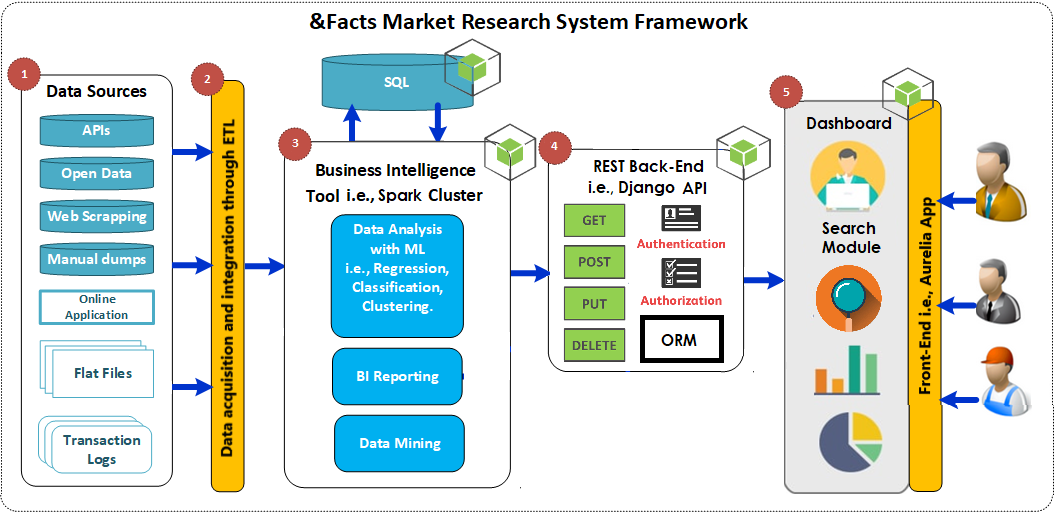
\includegraphics[scale=0.55]{img/systemarchitecture.png}
	\caption{System Architecture}
\end{figure} 

The conceptual view of the reference architecture shows the components of the \&Facts Market Research platform solution. The marketing research platform is made of:
\begin{itemize} 
	\item A Front-End Application made of a Dashboard component and a Search module;
	\item A Back-End REST Application orchestrating communication between modules and handling the session;
	\item A Business Intelligence Tool that performs data analysis and data mining and generates useful reports;
	\item A SQL database that holds the data of the platform;
	\item A Data Acquisition module that fetches data from the various sources;
	\item A Data Integration component that performs data integration through the ETL paradigm.
\end{itemize} 


\newpage
\section{Functional and Technical User Stories}
The project goal is to develop a web-based Minimum Viable Product (MVP) general purpose Market Research Platform integrating AI and Big Data technologies that will be running on the cloud. In order to build the \&Facts platform, the following steps are followed:
\begin{itemize} 
	\item The Front-end application will be written using Aurelia JS and Bootstrap. The application will run in a Docker container and will include a secure access module, updating and configuration capabilities, a search system and an intelligent marketing information visualization dashboard (using tables, graphs, and charts);
	\item The Back-end REST application will be developed using Python over Django and Spark. This component will reply to queries and perform disk-efficient and computationally optimized information gathering, data aggregation and analysis;
	\item The User Search module will take a list of keywords provided by the user and fetch them through appropriate APIs iteratively in order to generate more related keywords. The keywords  saved into a keystore as they are being generated. The main APIs that will be used for the implementation of this module are Facebook Graph API and DataforSEO;
	\item The Data Acquisition module will fetch relevant data from APIs given by the customer and other sources using the keywords generated by the User Search module. Different data sources should be used accordingly depending on the use case;
	\item The Data Integration module will map the retrieved data to a common structure, sort it, filter it and verify it using the ETL paradigm (Extract, Transform, Load). Duplicated rows may be removed from the data. Spark framework will be used for preprocessing huge data sets from multiple sources and as it can run on a cluster;
	\item The Business Intelligence tool-set will use AI and ML on the data to produce results such as forecasting, causal factors and economics of trends, classification of features and clustering, NLP analysis on Facebook ads, social listening and more;
	\item The data will be stored in a relational database that will be connected with the Data acquisition and Data integration modules on one end and the Business Intelligence tool-set on the other.
	\item The whole platform will be developed locally and continuously deployed inside Docker containers running on Amazon Web Services clusters;
\end{itemize} 
